\documentclass[12pt,a4paper]{article}

%\usepackage[german]{babel} %Für die indirekte Angabe von Umlauten. Es müssen dann Umlaute wie folgt im Code angegeben werden: "a "o "u "s.

\usepackage[utf8]{inputenc}
%dieses Paket ermöglicht uns, Umlaute im Text als solche eingeben zu können (Windows/Linux)

\usepackage{amsmath, amsthm, amssymb}
\usepackage{enumerate}
\usepackage{graphicx}
\usepackage{lscape}
\usepackage{setspace}
\onehalfspacing
\usepackage{wrapfig}
\usepackage{hyperref}% für die Einbettung von Hyperlinks
\usepackage{multirow}
\usepackage[round]{natbib}
\usepackage{longtable}
\bibliographystyle{apalike}

\newtheorem{definition}{Definition}[section]
\newtheorem{interview}{Interview}[section]
\newtheorem{satz}{Satz}[section]
\newtheorem{beispiel}{Beispiel}[section]
\newtheorem{bemerkung}{Bemerkung}[section]
\newtheorem{literaturverzeichnis}{Literaturverzeichnis}[section]

\usepackage[top=20mm, bottom=20mm, left=20mm, right=20mm, includehead]{geometry} % Document Margins
\setlength{\topmargin}{0cm}
\setlength{\parindent}{0mm}
\setlength{\parskip}{2mm}
\setlength{\evensidemargin}{0mm}
\setlength{\oddsidemargin}{0cm}
%\pagestyle{headings}

\providecommand{\tightlist}{%
  \setlength{\itemsep}{0pt}\setlength{\parskip}{0pt}}

\begin{document}
\thispagestyle{empty}
\vspace*{-3cm}
\begin{center}
\large \textsc{}
\vspace{0.5cm}
%\hrule
\vspace{5.5cm}
{\large}\\
\vspace{1cm}
{\Large \bf
Estimer la durée des tâches automatiquement}\\
\vspace*{1cm}
{\large avec l'arithmétique et l'intelligence artificielle}
\end{center}
\vspace*{14cm}


\hspace*{\fill} écrit par Stefan Hoffmann et des autres, \today

\newpage
\pagenumbering{Roman}
\tableofcontents

%\newpage
%\addcontentsline{toc}{section}{tables} %wenn es im Inhaltsverzeichnis erscheinen soll - sonst auskommentieren mit "%"
%\listoftables

%\newpage
%\addcontentsline{toc}{section}{Abbildungsverzeichnis} %wenn es im Inhaltsverzeichnis erscheinen soll - sonst auskommentieren mit "%"
%\listoffigures

\newpage
\pagenumbering{arabic}

\hypertarget{foreword}{%
\section{Foreword}\label{foreword}}

I want to make it short. Guessing task durations is a mess. You can put a lot of effort in making time estimates. Still they will be not good. And while you strife to make perfect estimates you will find yourself investing more and more time - possibly a lot more than the task is worth.

Unfortunately we cannot fully discard them, since guessing

With automation you can get more benefits and less pain:

\begin{itemize}
\tightlist
\item
  Since the algorithms are based on actual data, they are not "just wild guesses". They can watch a particular pipeline and become better and better according to the actual output.
\item
  Algorithms are systematic. They are well documented in terms of how they guess. This way they do not trigger the more human problems when guessing time estimates: The boss will half this guess, so I will better double it... The boss sees your estimate and cuts it down to 15 Minutes because "what could be the problem?".
\item
  Because of works like this e-book and scientific methods available to us algorithms can be validated. This means we can become better and better.
\item
  It is more easy to communicate, that it is a guess, not a fixed date. The algorithms will give you a number. It does not know what it is actually guessing. 
\item
  Business people can have their time estimates in nearly real time.
\item
  The developers of those business peoples can do other things in the time they would spend guessing. For example they can code. This means they are more productive.
\item
  The developers are more happy because they do not loose time to guessing and they have no need to fight all the people off that ask for an estimate just to ridicule it and then punish developers for not reaching the deadline that they faked. 
\end{itemize}

Let us see, if the idea is working or not. Maybe not. But, since the only thing we have to loose is bad estimates and the only thing we can gain is bad estimates that do not make effort - what the heck.

\hypertarget{accompagning-material}{%
\section{Accompagning Material}\label{accompagning-material}}

With this booklet I release:

\hypertarget{estimateps}{%
\subsection{EstimatePS}\label{estimateps}}

EstimatePS is a powershell commandlet to estimate tasks from the command
line, implemented but not limited to Powershell Core. The code is part
of this repository. But it is also available through the Powershell
Gallery.

\begin{verbatim}
Install-Module EstimatePS
\end{verbatim}

May it be of service for those in need.

\newpage{}

\hypertarget{quality-assurance}{%
\section{Quality Assurance}\label{quality-assurance}}

Now if we create algorithms we need to say how good they are. For that
we are using the following methods.

\hypertarget{the-graphical-approach}{%
\subsection{The graphical approach}\label{the-graphical-approach}}

One easy way would be to draw a graph which shows the predictions and
the real values for time spent, while each task is understood as a
category of its own.

We sort that graph by actual duration so we should see the distribution
of durations and around that a hopping range of dots that describes what
the algorithm tells us.

A better algorithm should be closer to the real data. Any algorithm
should never match perfectly, as then we would have a 1:1 mapping. And
that is an over-fit for sure.

\hypertarget{mean-squared-error}{%
\subsection{Mean squared error}\label{mean-squared-error}}

The mean squared error is a common approach to calculate a value for the
quality of an algorithmi. It gets bigger with every estimate we did
wrong.

The formula can be described as:

For every value you predict:

\begin{itemize}
\tightlist
\item
  Calculate the difference between the predicted value and the real
  value
\item
  Sum the squares of each difference
\item
  Divide all the sum by the count of the data entries you check
\end{itemize}

Now, since we want to prevent overfitting we need to prevent
underfitting as well. Since we are talking about seconds and most of the
recorded tasks have a duration in the range of up to 50000 seconds that
means that most tasks are completed in about 13,89 hours. So what about
an error margin of about 5 hours. Which means just as something to think
of, we want the squared error to not exceed squared(5x60x60) =
324.000.000 .

\hypertarget{above-and-below}{%
\subsection{Above and below}\label{above-and-below}}

As a third criteria we have the idea that estimations might even each
other out. In a prefect scenario this would mean that 50\% of the
estimations are too high while the other 50\% are too low. To find out
how good we match we add 1 to a variable for every estimation we find
above the real value and then divide it by the number of tasks. The
result should be .5 when hitting the target.

\hypertarget{the-data}{%
\subsection{The Data}\label{the-data}}

For training and estimating the quality of algorithms I use herein a
dataset that consists of all the tasks that we at the software
development shop at my employer recorded during the time between july
and december 2020 and january 2021 to august 2021. That means there are
two datasets available.

Unfortunately - since this is confidential information - I cannot
publish it alongside this material. But the errors and images can be
shared at it can advance the algorithms - and it is everything that I
have right now. So that will do.

I'll call them: swe2020 and swe2021.

Now let us get a glance at the data as well the first algorithm.


\newpage{}

\hypertarget{a001---duration-per-word}{%
\section{A001 - Duration per Word}\label{a001---duration-per-word}}

\hypertarget{description}{%
\subsection{Description}}

Let us dive in with a very very simple algorithm. In fact it is the
first algorithm I tought of.

Let's say we have a task. May it read ``Buy a big book and put it in the
shelf''. And this takes a certain amount of time.

\begin{verbatim}
AmountOfTime = "Buy a big book and put it in the shelf"
\end{verbatim}

Ok, I know, language doesn't really work like that. But lets us play
stupid right now. We just split the thing into words and distribute the
duration equally to each word. The sentence above is 10 words long, so
each word gets a tenth of AmountOfTime associated with it.

Now we have a minimal time table.

We can now take another input, like ``Buy a small book''.

We know the durations associated with ``Buy'', ``a'' and ``book''. We
will have to do something about the unknown word. Ignore it, or add 10\%
to the sum of the known durations. Something like that. And voilà, we
have a time estimate.

Funny thing:

It is actually quite reasonable for the time being, that, in the absence
of further information, assigning half the duration to each subtask is
not the most stupid thing one could do.

And it is actually quite reasonable to think that buying a small book is
about the effort of buying a big one. But that is just the example.

Anyways, we now have a time estimate and noone got hurt.

\hypertarget{using-the-algorithm-from-powershell}{%
\subsection{Using the algorithm from powershell}}

The algorithm is added to EstimatePS, see
Source/experiments/duration-per-word/experiment1.ps1 for a complete
example with learning, caching and usage.

Finally it is as easy as:

\begin{verbatim}
$inSeconds = Get-DPWEstimate -Model $model -DurationInSecondsFor "add a new bookkeeping api" -ProbabilityInPercent 95
\end{verbatim}


\newpage{}
\newpage{}

\hypertarget{a002---simply-an-average}{%
\section{A002 - Simply an average}\label{a002---simply-an-average}}

\hypertarget{description}{%
\subsection{Description}}

Another algorithm could just calculate an average. Take all tasks and
their durations, divide them by their count. Is this better?

From visually reviewing the data we know that most tasks have a duration
of a few hours max. Some take very long.

An average is not just an average as we know. There are several ways to
calculate one:

\begin{itemize}
\tightlist
\item
  there is the ``simple average'' that includes all data (A002.1)
\item
  there is the possibility of a boxplot like calculation, include only
  the middle n\% of the values (A002.2)
\end{itemize}

\hypertarget{using-the-algorithm-from-powershell}{%
\subsection{Using the algorithm from powershell}}

\hypertarget{a002.1}{%
\subsubsection{A002.1}}

Have a look at Quality-Assurance\_A002\_1\_swe2020.ps1 if you need more.
But actually it is just calculating the average. It is not even
necessary to do this in a programming language alltogether.

\begin{verbatim}
$averageTaskDuration = ($historicData.DurationInSeconds | Measure-Object -Average).Average

$anyEstimation = $averageTaskDuration
\end{verbatim}

\hypertarget{a002.2}{%
\subsubsection{A002.2}}

For that average let us only use the middle 90\% of duration values.
That will cut extreme points and should reduce the error.

Quality-Assurance\_A002\_2\_swe2020.ps1:

\begin{verbatim}
$historicData = $historicData | Sort-Object DurationInSeconds
$count = ($historicData | Measure-Object).Count
$fivePercent = [int]($count * 0.05)
$historicData = $historicData[$fivePercent..($count-$fivePercent)]
\end{verbatim}


\newpage{}

\hypertarget{a003---10-categories}{%
\section{A003 - 10 catégories}\label{a003---10-categories}}

\hypertarget{description}{%
\subsection{Description}}

Pour faire mieux que A001 on peux utiliser des catégories. 
Les tâches sont divisés en 10 groupes qui ont des proprieté differentes.
Le but est de réduire la dispersion dans la catégorie des tâches de moins d'une heure.
Mais comment ce faire?

\subsubsection{A003.1}

On crée un barème linéar pour les tâches qui sont 
\begin{enumerate}
\tightlist
\item inférieures à 30 minutes,
\item supérieures à 30 minutes et inférieures à une heure,
\item supérieures à une heur et inférieures à deux heures
\item supérieures à 2 heures et inférieures à 3 heures
\item supérieures à 3 heures et inférieures à 4 heures
\item supérieures à 4 heures et inférieures à 5 heures
\item supérieures à 5 heures et inférieures à 6 heures
\item supérieures à 6 heures et inférieures à 7 heures
\item supérieures à 7 heures et inférieures à 8 heures
\item supérieures à 8 heures
\end{enumerate}

Notre algorithme pour apprendre les mots qui sont signifiqative par catégorie c'est ca:
\begin{enumerate}
\tightlist
\item on recueille tous les mots par catégorie
\item pour toutes les catégories:
    \begin{enumerate}
        \tightlist
        \item soustraire tous les mots qui font partie d'une autre catégorie
    \end{enumerate}
\end{enumerate}






\newpage{}

\hypertarget{a004---reducing-dispersion-by-assigning-a-concrete-value-per-word-and-learning-from-it}{%
\section{A004 - reducing dispersion by assigning a concrete value per
word and learning from
it}\label{a004---reducing-dispersion-by-assigning-a-concrete-value-per-word-and-learning-from-it}}

A001 collects as many different values for each word as it can get. When
estimating, it uses any of those values more or less randomly (of cause
smoothend by the fact that we take 100 random values and then only use a
value from a certain position representing the percentage of certainty
we want to have). Anyways, that hinders our ability to ``learn''.

The idea behind this algorithm is to assign just one value to each word.
This way, when we see our error margin we might design a little learning
algorithm.

For example: - create an average model - while the mean squared error is
higher than \ldots{} - create 10 mutation of that model, for example by
randomly adding or substracting 1/10th of the value to each weight of
each word. - calculate the mean squared error for each mutation - take
the model with the least mean squared error and repeat


\newpage{}

\begin{landscape}

\hypertarget{results-per-algorithm}{%
\section{Results Per Algorithm}\label{results-per-algorithm}}

\subsection{Overview}

\begin{tabular}{lllrr}
\hline
 Algorithm   & Training on   & Estimating    &   with params &                 deviation \\
\hline
 A001        & SWEArchiv2020 & SWEArchiv2020 &         25\%P &  -1.277 $\pm$ 6.822 hours \\
 A001        & SWEArchiv2020 & SWEArchiv2020 &         50\%P &  -0.900 $\pm$ 6.369 hours \\
 A001        & SWEArchiv2020 & SWEArchiv2020 &         75\%P &   0.099 $\pm$ 6.097 hours \\
 A001        & SWEArchiv2020 & SWEArchiv2020 &         80\%P &   0.453 $\pm$ 5.573 hours \\
 A001        & SWEArchiv2020 & SWEArchiv2020 &         90\%P &   2.057 $\pm$ 5.626 hours \\
 A001        & SWEArchiv2020 & SWEArchiv2020 &        100\%P &  -1.829 $\pm$ 7.691 hours \\
 A001        & SWEArchiv2020 & SWEArchiv2021 &         25\%P & -1.546 $\pm$ 12.133 hours \\
 A001        & SWEArchiv2020 & SWEArchiv2021 &         50\%P & -1.320 $\pm$ 12.129 hours \\
 A001        & SWEArchiv2020 & SWEArchiv2021 &         75\%P & -0.675 $\pm$ 12.127 hours \\
 A001        & SWEArchiv2020 & SWEArchiv2021 &         80\%P & -0.345 $\pm$ 12.195 hours \\
 A001        & SWEArchiv2020 & SWEArchiv2021 &         90\%P &  0.805 $\pm$ 12.232 hours \\
 A001        & SWEArchiv2020 & SWEArchiv2021 &        100\%P & -1.744 $\pm$ 12.136 hours \\
 A002\_1     & SWEArchiv2020 & SWEArchiv2020 &               &  -0.000 $\pm$ 7.691 hours \\
 A002\_1     & SWEArchiv2020 & SWEArchiv2021 &               &  0.085 $\pm$ 12.136 hours \\
 A002\_2     & SWEArchiv2020 & SWEArchiv2021 &        L75\%M &  -0.326 $\pm$ 7.691 hours \\
 A002\_2     & SWEArchiv2020 & SWEArchiv2021 &        L85\%M &   0.188 $\pm$ 7.691 hours \\
 A002\_2     & SWEArchiv2020 & SWEArchiv2021 &        L95\%M &   0.214 $\pm$ 7.691 hours \\
\hline
\end{tabular}

\end{landscape}
\newpage
\subsection{Box-Plots INPUT/OUTPUT for the lower 90\% of tasks}

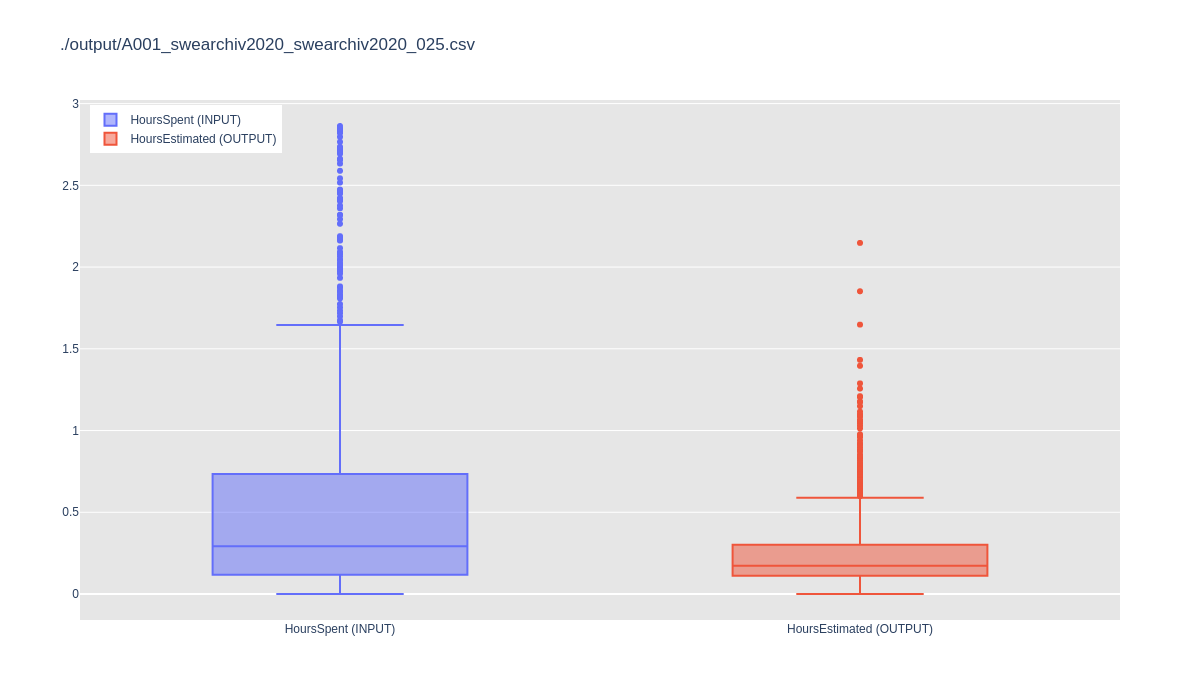
\includegraphics[width=\textwidth]{Scripts/output/A001_swearchiv2020_swearchiv2020_025.csv.png}
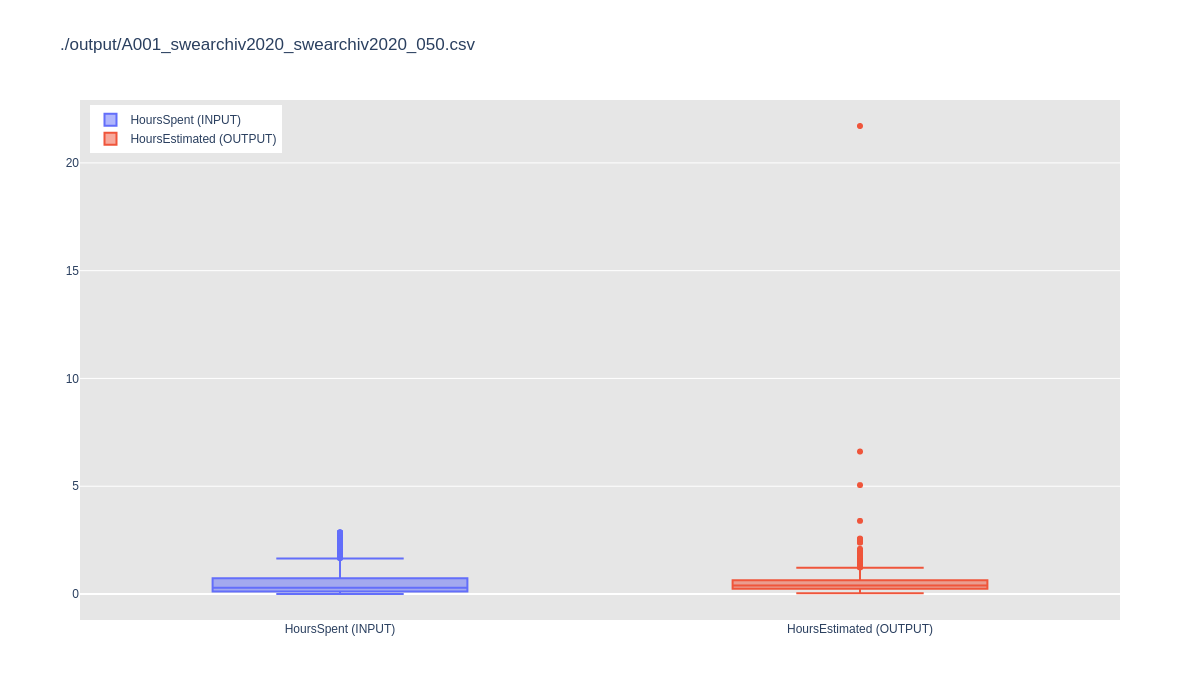
\includegraphics[width=\textwidth]{Scripts/output/A001_swearchiv2020_swearchiv2020_050.csv.png}
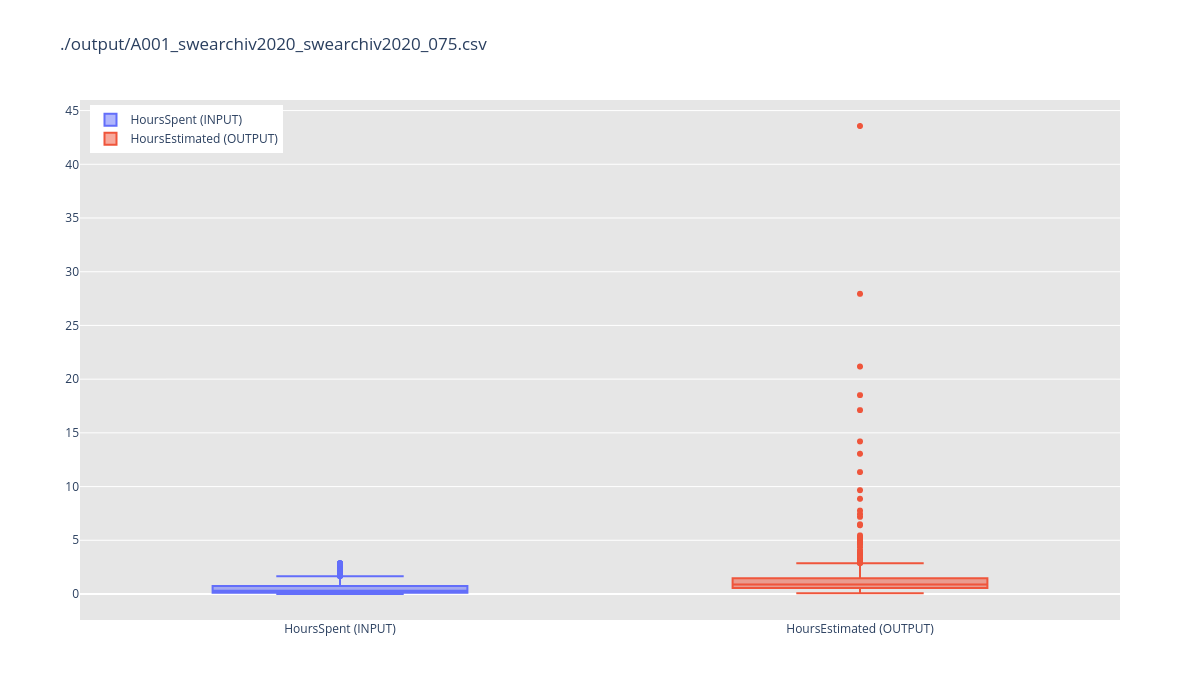
\includegraphics[width=\textwidth]{Scripts/output/A001_swearchiv2020_swearchiv2020_075.csv.png}
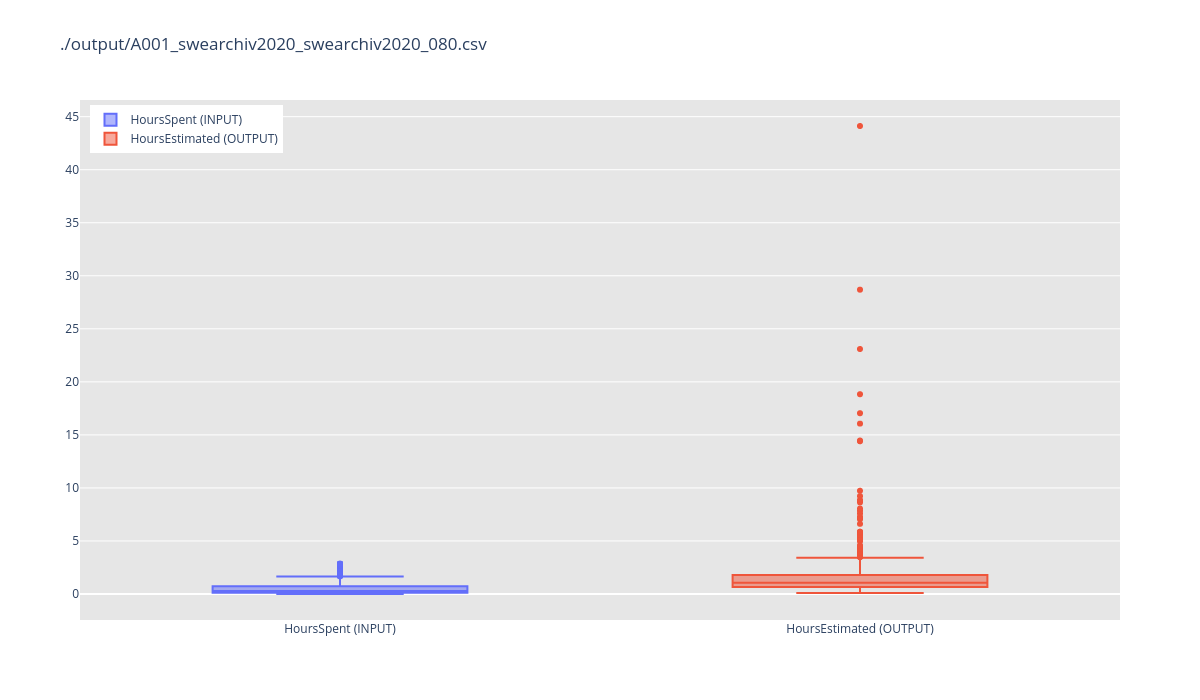
\includegraphics[width=\textwidth]{Scripts/output/A001_swearchiv2020_swearchiv2020_080.csv.png}
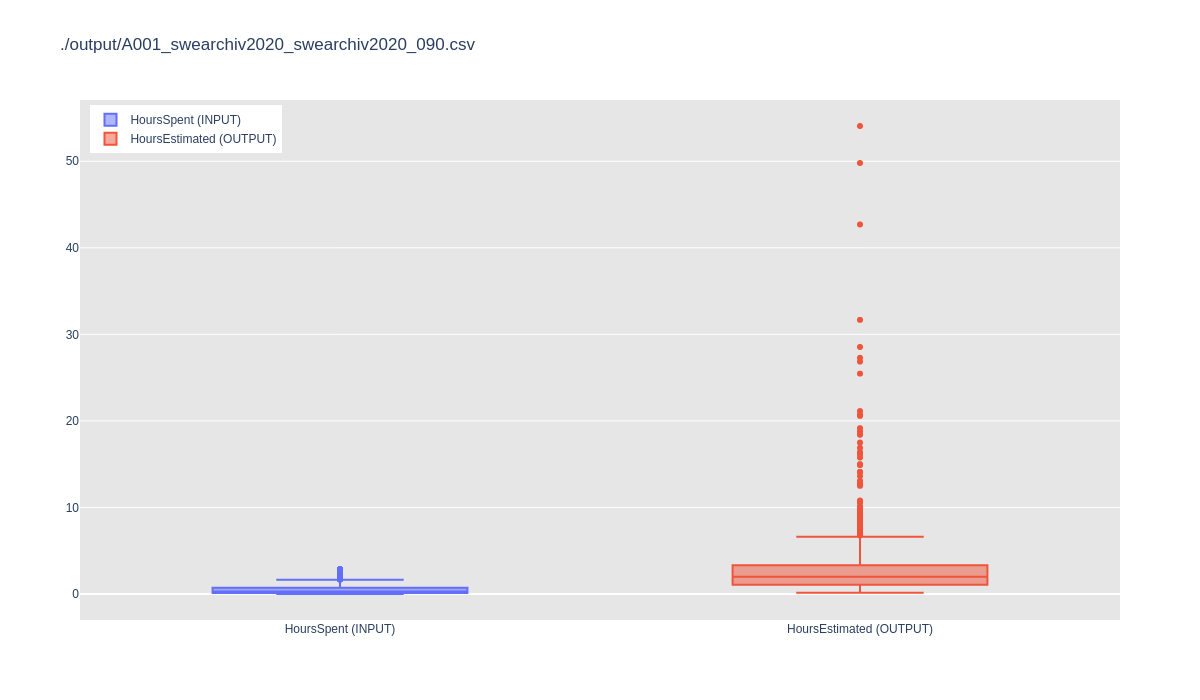
\includegraphics[width=\textwidth]{Scripts/output/A001_swearchiv2020_swearchiv2020_090.csv.png}
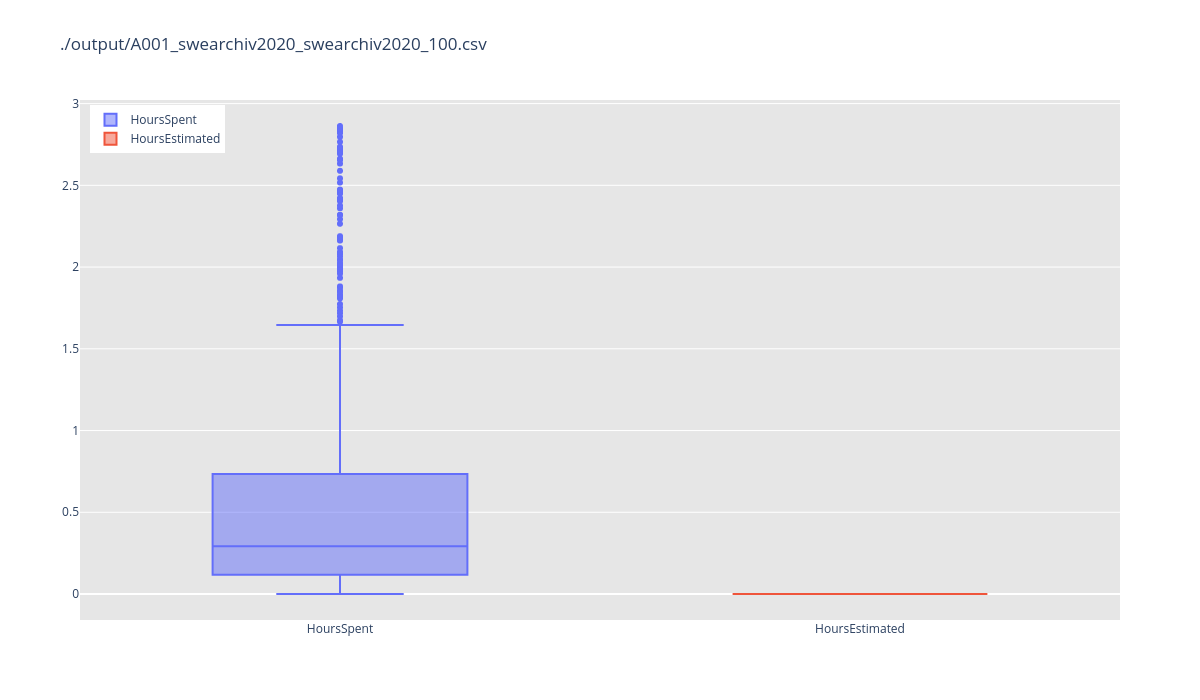
\includegraphics[width=\textwidth]{Scripts/output/A001_swearchiv2020_swearchiv2020_100.csv.png}
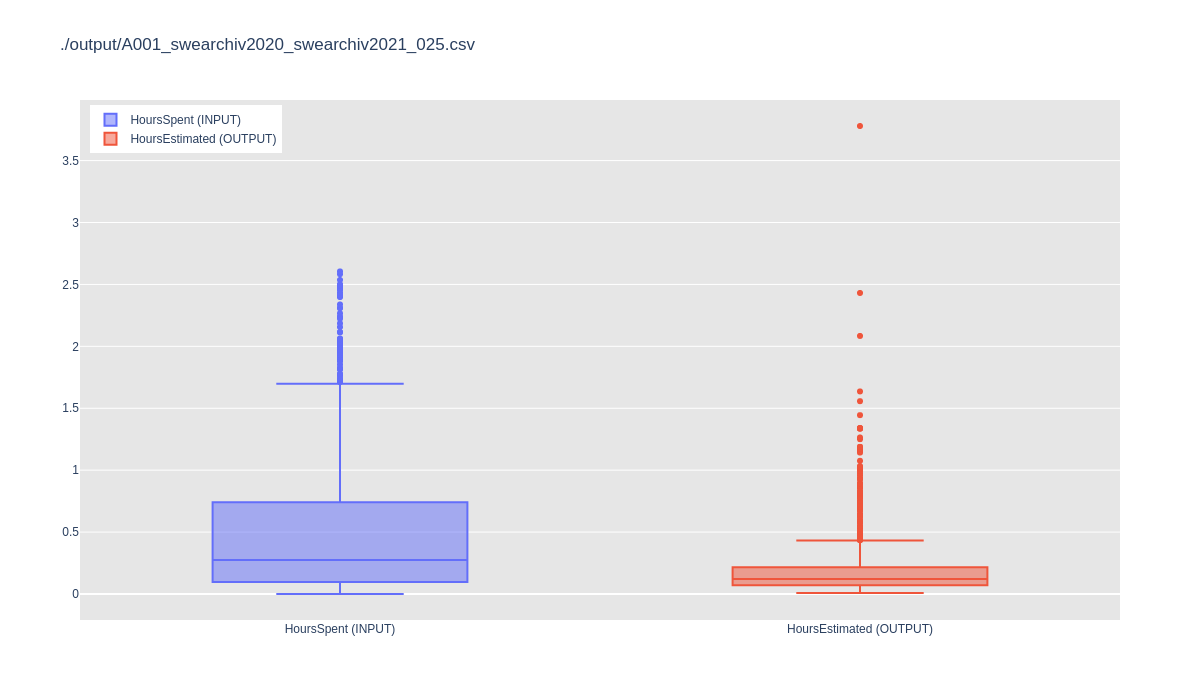
\includegraphics[width=\textwidth]{Scripts/output/A001_swearchiv2020_swearchiv2021_025.csv.png}
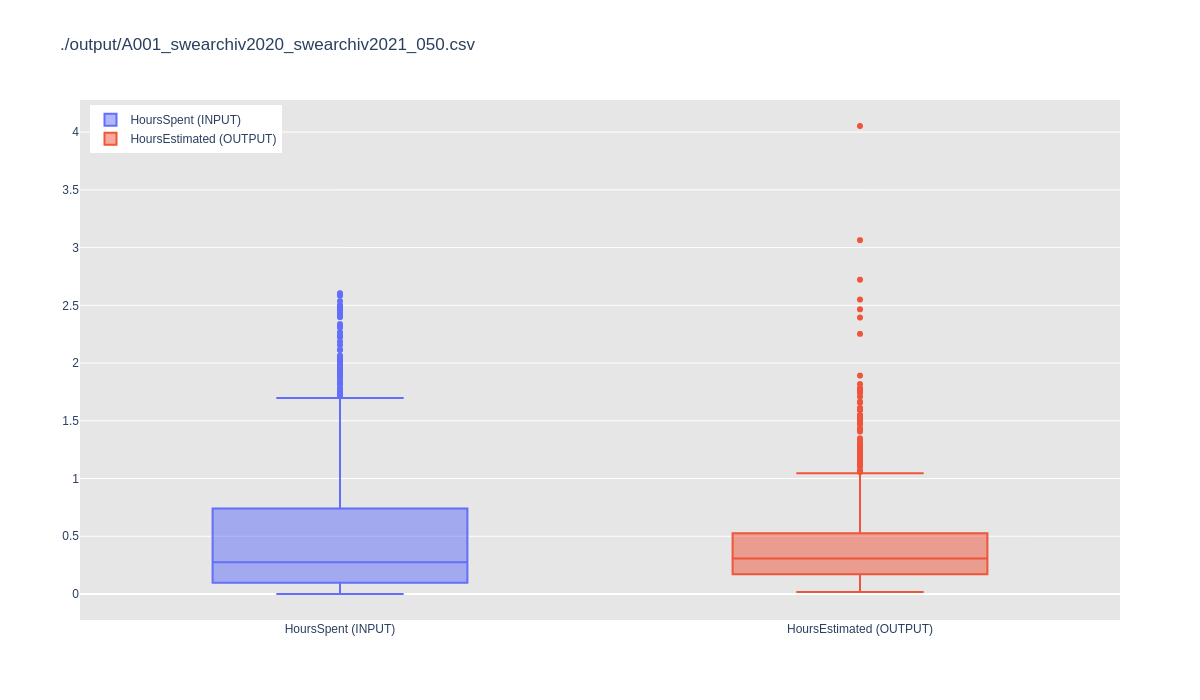
\includegraphics[width=\textwidth]{Scripts/output/A001_swearchiv2020_swearchiv2021_050.csv.png}
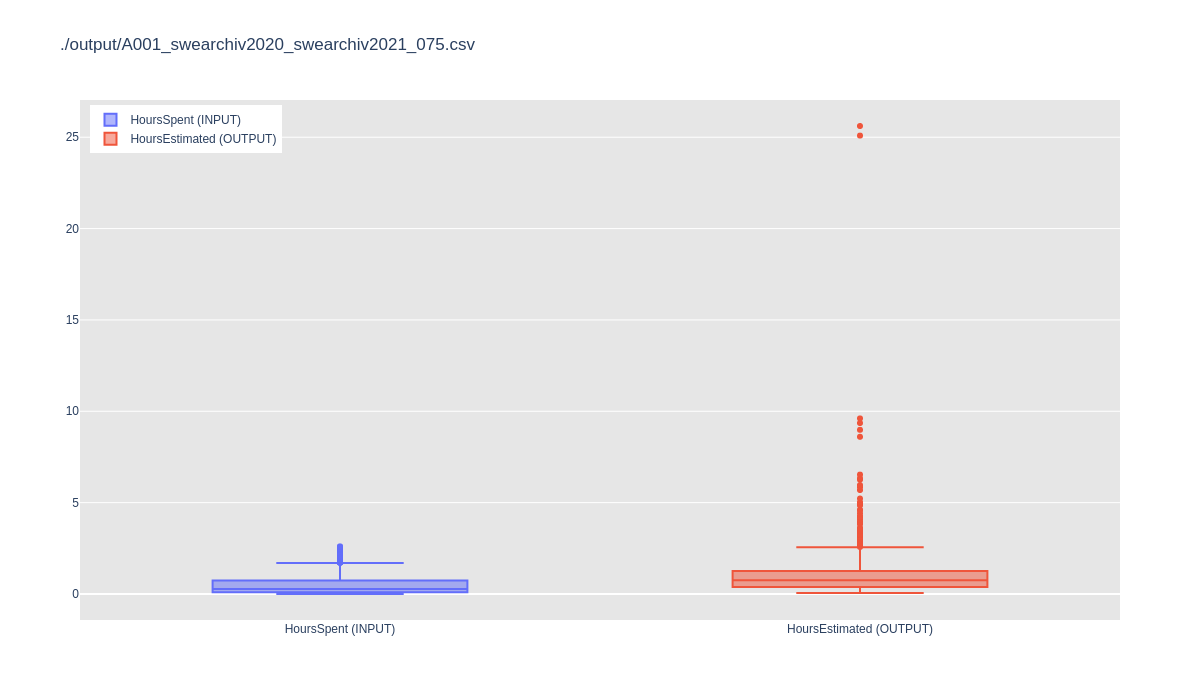
\includegraphics[width=\textwidth]{Scripts/output/A001_swearchiv2020_swearchiv2021_075.csv.png}
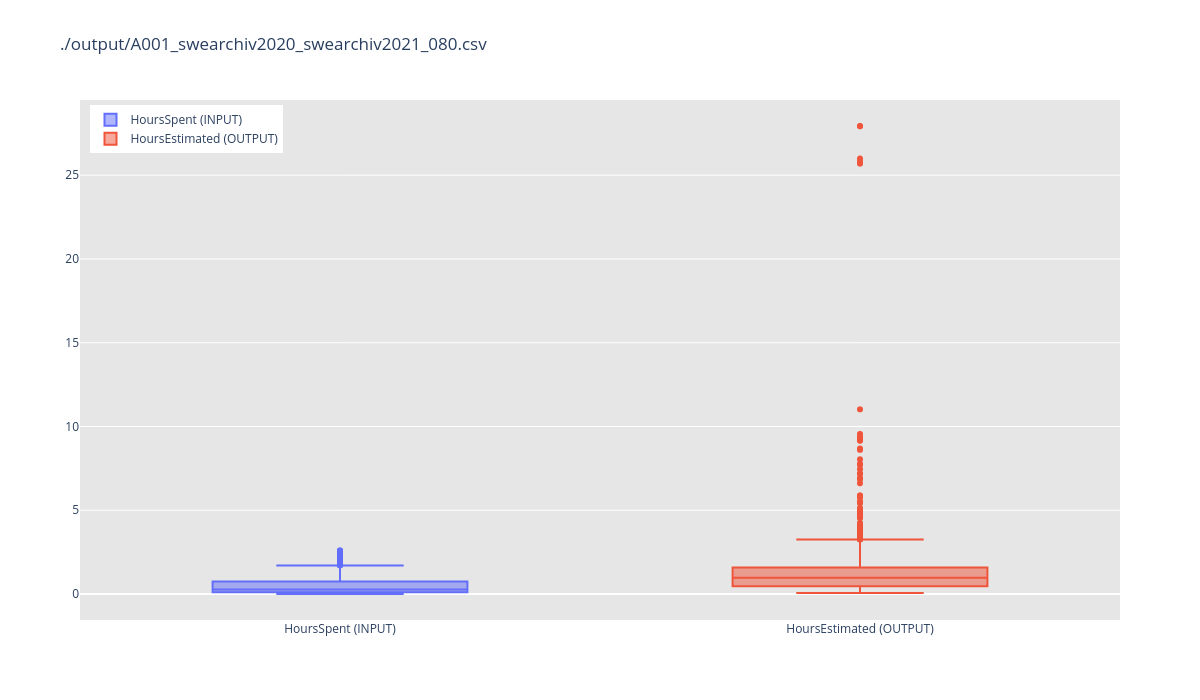
\includegraphics[width=\textwidth]{Scripts/output/A001_swearchiv2020_swearchiv2021_080.csv.png}
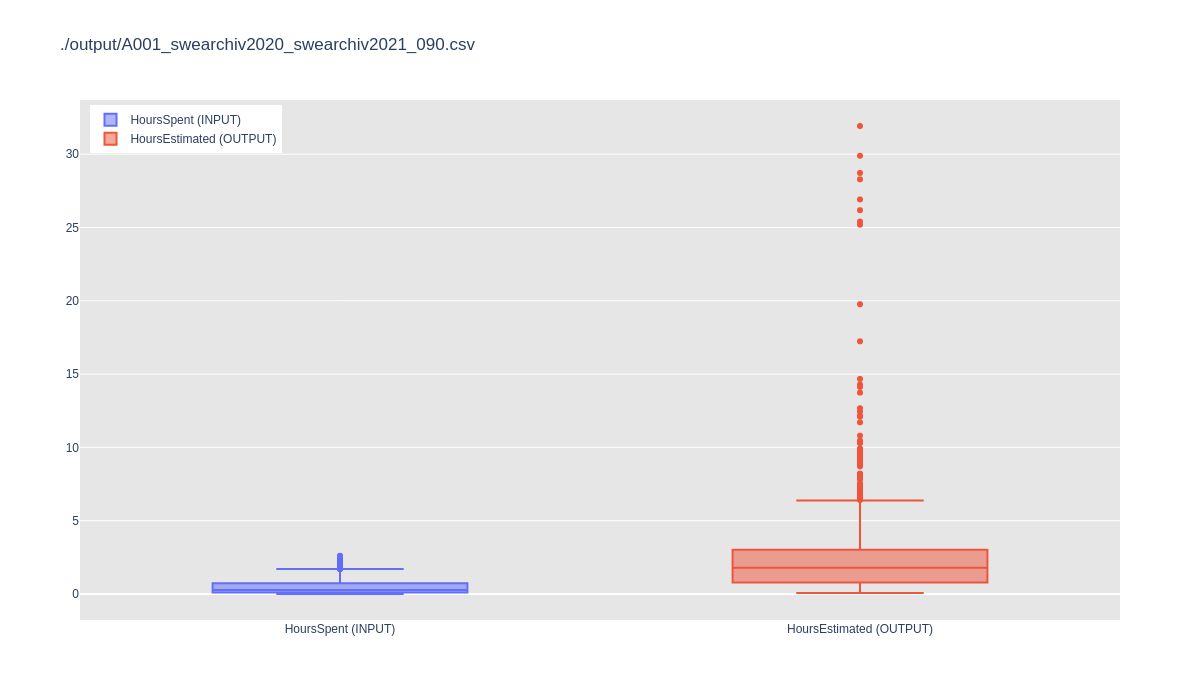
\includegraphics[width=\textwidth]{Scripts/output/A001_swearchiv2020_swearchiv2021_090.csv.png}
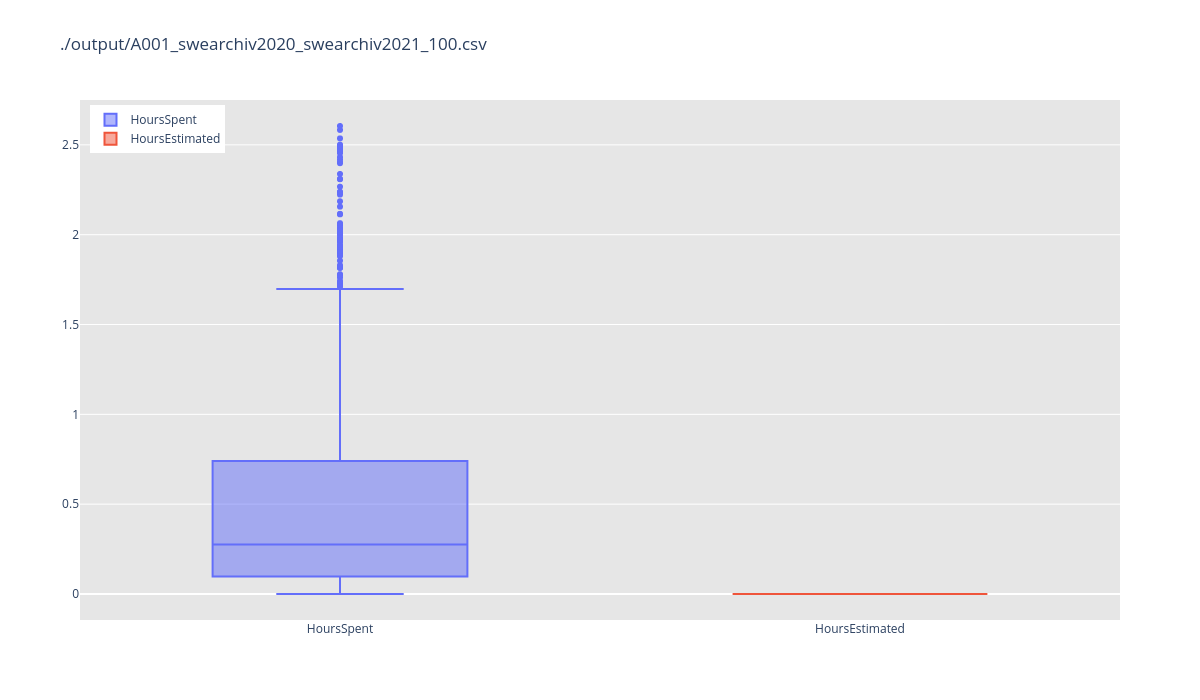
\includegraphics[width=\textwidth]{Scripts/output/A001_swearchiv2020_swearchiv2021_100.csv.png}




\end{document}

